% ex: ts=2 sw=2 sts=2 et filetype=tex
% SPDX-License-Identifier: CC-BY-SA-4.0
\begin{frame}
    \frametitle{Contenido}
    \tableofcontents
\end{frame}

\section{Concepto de algoritmo}

\begin{frame}[c]{Definición de algoritmo}
  \begin{block}{Definición}
    \begin{itemize}
      \item Conjunto ordenado y finito de operaciones que permite hallar
            la solución de un problema\footnote{Real academia española}.
      \item Conjunto de pasos, acciones o instrucciones necesarios para
            lograr un resultado o resolver un problema.
      \item Secuencia ordenada de pasos exentos de ambigüedad tal que, al
            llevarse a cabo con fidelidad, dará como resultado que se realice
            la tarea para la que se ha diseñado en un tiempo finito.
    \end{itemize}
  \end{block}
\end{frame}

\begin{frame}[c]{Propiedades de un algoritmo}
  \begin{description}
    \item[Finitud] La ejecución de un algoritmo ha de terminar después de un
      número finito de etapas.
    \item[Precisión] Cada etapa ha de estar especificado rigurosamente. La
      ejecución de un algoritmo no ha de dejar espacio para la interpretación,
      la intuición o la creatividad.
    \item[Ordenado] Las instrucciones se ejecutan una después de otra en un
      orden específico. Al cambiar el orden, puede cambiar el resultado.
    \item[Definido] Cada instrucción atiende un solo problema particular.
      No se presta a ambigüedades (dobles significados).
  \end{description}
\end{frame}

\begin{frame}[c]{Características de un algoritmo}
  \begin{description}
    \item[Entradas] Un algoritmo tiene cero o más entradas (cantidades que se
      le dan inicialmente antes de que comience su ejecución).
    \item[Salidas] Un algoritmo tiene una o más salidas (cantidades que tienen
      una relación especifica con las entradas).
  \end{description}
  \begin{center}
    
\includegraphics[scale=0.5]{01-entradas-salidas.png}
  \end{center}
\end{frame}

\section{Resolución de problemas}

\begin{frame}[c]{Resolución de problemas por computadora}
  \begin{itemize}
    \item Descripción del problema (especificar lo que se pretende resolver).
    \item Análisis del problema (descripción de la funcionalidad del programa.
      Características, entradas y salidas, cálculos, tipos de datos,
      restricciones, etc.
    \item Diseñar un algoritmo para el problema.
    \item Expresar el algoritmo como un programa (codificación del algoritmo
      diseñado en un lenguaje de programación).
    \item Ejecutar el programa (pruebas y depuración de errores).
  \end{itemize}
\end{frame}

\begin{frame}[c]{Resolución de problemas por computadora}
  \begin{center}
    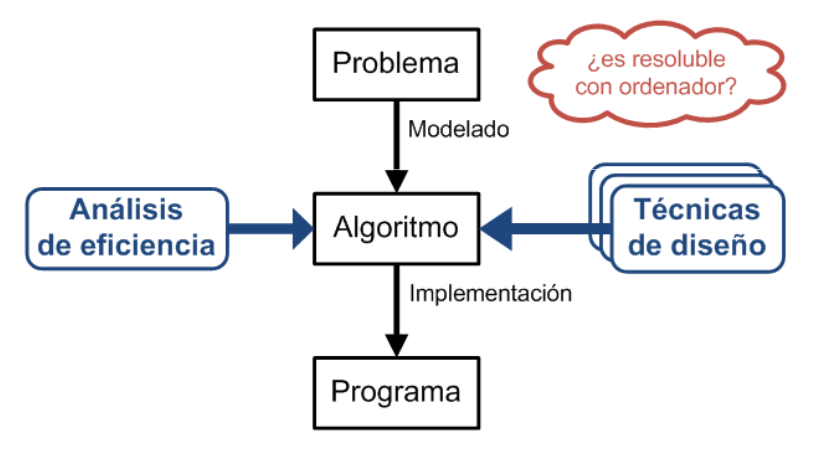
\includegraphics[scale=0.4]{01-problema-programa.png}
  \end{center}
\end{frame}

\section{Clasificación de problemas}

\begin{frame}[c]{Atreves de los años}
  \begin{description}
    \item[Años 30] Problemas computables y no computables.
    \item[Años 50] Complejidad de los problemas computables (búsqueda de
      algoritmos más eficaces).
    \item[Años 70] Clasificación de los problemas computables: \textbf{P}
      y \textbf{NP}
  \end{description}
\end{frame}

\begin{frame}[c]{Clases P y NP}
  \begin{description}
    \item[Clase P] Problemas resolubles en un tiempo polinómico con una máquina
      de Turing determinística (esto es, el tiempo de ejecución del algoritmo en
      un ordenador viene descrito por una fórmula polinómica).
    \item[Clase NP] \textbf{Non-Deterministic Polynomial-time} Problemas
      resolubles en tiempo polinómico con una máquina de Turing \textbf{no
      determinística}
  \end{description}
\end{frame}

\begin{frame}[c]{Clase $P \subseteq $ Clase $ NP$}
  \begin{center}
    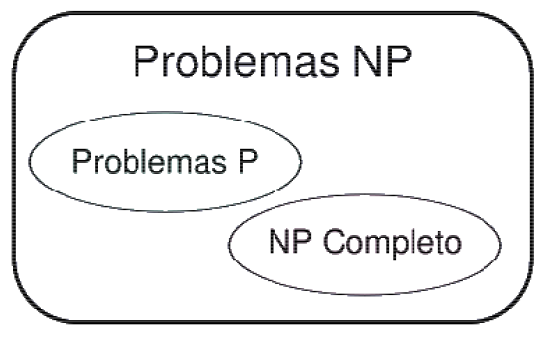
\includegraphics[scale=0.4]{01-problemas-np.png}
  \end{center}
\end{frame}

\begin{frame}[c]{Reducción de problemas y complejidad}
  \begin{itemize}
    \item Si reducimos un problema (A) a otro (B), podemos obtener una solución
      con un algoritmo para el problema B y transformar esa solución para
      convertirla en una solución para el problema A.
    \item \textbf{¿P = NP?} Si encontráramos un algoritmo polinómico para un
      problema \textit{NP-completo}, sabríamos que todos los problemas de clase
      NP se pueden resolver en tiempo polinómico.
  \end{itemize}
\end{frame}

\section{Algorítmica}

\begin{frame}[c]{Título}
    \begin{center}
        Texto
    \end{center}
\end{frame}

\section{Análisis de la eficiencia de los algoritmos}

\begin{frame}[c]{Título}
    \begin{center}
        Texto
    \end{center}
\end{frame}

\section{}

\begin{frame}[c]{Título}
    \begin{center}
        Texto
    \end{center}
\end{frame}

\section{Técnicas de diseño de algoritmos}

\begin{frame}[c]{Título}
    \begin{center}
        Texto
    \end{center}
\end{frame}
